\documentclass{article}
\usepackage{amsmath}
\usepackage{amssymb}

\usepackage{newtxtext}
\usepackage[varvw]{newtxmath} 

\usepackage{physics}
\usepackage{geometry}
\usepackage{tikz}
\usepackage{amsmath}
\usepackage{graphicx}
\usepackage{appendix} %%!!!!!!!!

\usetikzlibrary{fadings}
\usetikzlibrary{patterns}
\usetikzlibrary{shadows.blur}
\usetikzlibrary{shapes}

\geometry{b5paper}
\linespread{1.5}

%personalized symbols
%\newcommand{\dd}{\mathrm{d}}
\newcommand{\ii}{\mathrm{i}}
\newcommand{\ee}{\mathrm{e}}

\title{Seiberg-Witten Theory and Instanton Partition Function}
\author{Yilu Shao\\ \footnotesize{\it Department of Physics and Center for Field Theory and Particle Physics, Fudan University,}\\ \footnotesize{\it Shanghai 200433, China}}
\date{}

\setcounter{tocdepth}{1}

\begin{document}
\maketitle

\tableofcontents
\newpage

\begin{abstract}
We will give a pedagogical review of the Seiberg-Witten theory on 4d $\mathcal{N}=2$ supersymmetric gauge theory and briefly introduce Nekrasov's instanton counting method.

This is an on-going work based on my undergraduate thesis, and I will keep updating
\end{abstract}


\section{Briefs on 4d $\mathcal{N}=1$ Theories}

\section{Lagrangian for 4d $\mathcal{N}=2$ Theories}
In this section, we will construct the Lagrangian for 4d $\mathcal{N}=2$ pure Yang-Mills theory in the language of $\mathcal{N}=1$ theories. We will see that the superfield formalism of 4d $\mathcal{N}=1$ theories only works partially in 4d $\mathcal{N}=2$ theories.

\subsection{Supercharges}
The concept of $\mathcal{N}=2$ means we need to introduce $8$ supercharges $\mathcal{Q}$ in the theory. These supercharges are Weyl spinors that obey the following commutation relation
\begin{equation}
\left\{\mathcal{Q}_{\alpha}^{I}, \bar{\mathcal{Q}}_{\dot{\alpha} J}\right\}=2 \delta_{J}^{I} \sigma_{\alpha \dot{\alpha}}^{\mu} P_{\mu}, \quad\left\{\mathcal{Q}_{\alpha}^{I}, \mathcal{Q}_{\beta}^{J}\right\}=\epsilon_{\alpha \beta} \epsilon^{I J} Z, \quad\left[\mathcal{Q}_{\alpha}^{I}, P_{\mu}\right]=0. 
\end{equation}
In which $I,J=1,2$ labels different supercharges. Here $\alpha$ and $\dot{\alpha}$s are spinor indices. $P_{\mu}$ is the translation generator and $Z$ is called the central charge. 

This theory admits an $\mathfrak{su}(2)_R\times U(1)_r$ R-symmetry if we treat the supercharge $\mathcal{Q}$ (or $\bar{\mathcal{Q}}$) as a left (right) hand Weyl spinor. The $\mathfrak{su}(2)_R$ act on the spin-$1/2$ doublet of supercharges as
\begin{equation}
SU(2)_R\circlearrowright\begin{pmatrix}
\mathcal{Q}^1_{\alpha}\\
\mathcal{Q}^2_{\alpha}\\\end{pmatrix}
\end{equation}
In general, the $\mathfrak{u}(1)_r$ is anomalous, but it is non-anomalous in an SCFT.

\subsection{$\mathcal{N}=2$ Supermultiplets}
Now we consider the supersymmetric multiplets in $\mathcal{N}=2$ theories with gauge group $\mathfrak{g}$. In analogy with the $\mathcal{N}=1$ case, pure Yang-Mills theories can have only vector multiplets, and the hypermultiplets somehow stand for matters.

\subsubsection{Vector Multiplet}
Unlike the $\mathcal{N}=1$ case, the $\mathcal{N}=2$ vector multiplet is composed of four fields (if we omit auxiliary ones), which can be regarded as a $\mathcal{N}=1$ chiral multiplet and a $\mathcal{N}=1$ vector multiplet, all of them are in adjoint representation.
\begin{equation}
\mathcal{N}=2\ \text{Vector multiplet}\;V :\ \left\{
\begin{matrix}
 &A^{A}_{\mu}& \\
\eta_{\alpha}^A& &\lambda_{\alpha}^A
\\&\phi^A& 
\end{matrix}
\right.
\end{equation}
here $\phi$ is the scalar field, $A_\mu$ the gauge field and $\eta,\lambda$ the gaugino. Since they are all in adjoint representation, the latin indices $A=1,...,\mathrm{dim}\mathfrak{g}$. Fields on the same row have the same $R$-charge and the same spin in the same column.

The $\mathcal{N}=2$ vector multiplet $V^{\mathcal{N}=2}$ can be written in the language of $\mathcal{N}=1$ theory as $(\Phi, V^{\mathcal{N}=1})$, where $\Phi$ consists of $\phi$ and $\eta$, and $ V^{\mathcal{N}=1}$ contains $\lambda$ and $A_\mu$. Inside the $\mathcal{N}=1$ multiplets $\phi$ and $\eta$, $\lambda$ and $A_\mu$ are related by supercharge $\mathcal{Q}^1$, while $\phi$ and $\lambda$, $\eta$ and $A_\mu$ are related by $\mathcal{Q}^2$. 

\subsubsection{Hypermultiplet}
$\mathcal{N}=2$ hypermultiplet can be decomposed into a $\mathcal{N}=1$ chiral multiplet and a $\mathcal{N}=1$ anti-chiral multiplet.
\begin{equation}
\mathcal{N}=2\ \text{Hypermultiplet}\;\Phi:\ \left\{
\begin{matrix}
 &\tilde{\psi}^{\dagger i}_{\alpha}& \\
q^i& &\tilde{q}^{\dagger i}
\\&\psi_{\alpha}^i& 
\end{matrix}
\right.
\end{equation}
The index $i=1,...,N_f$ marks the flavor. $q$ and $\psi_\alpha$ forms a chiral multiplet $Q$ and so is $\tilde{q}^{\dagger}$ and $\psi^{\dagger}_\alpha$ in anti-chiral multiplet $\tilde{Q}^{\dagger}$. 

$q$ and $\tilde{q}^{\dagger}$ forms a $SU(2)_R$ doublet
\begin{equation}
\begin{pmatrix}
q\\
\tilde{q}^{\dagger}\\\end{pmatrix}\circlearrowright SU(2)_R
\end{equation}
which means $SU(2)_R$ can rotate $\mathcal{N}=1$ chiral multiplet $Q$ and anti-chiral multiplet $\tilde{Q}^{\dagger}$.

\subsection{Lagrangians}
\label{Lagrangians}
Now we can write down the Lagrangian for $\mathcal{N}=2$ theories, for pure Yang-Mills
\begin{equation}
\mathcal{L}_{\mathrm{vect.}}=\frac{\tau}{16\pi \mathrm{i}} \int \mathrm{d}^{2} \theta\left(\frac{1}{2} \mathrm{tr} W^{2}+\mathrm{h.c.}\right)
+\frac{\operatorname{Im}\tau}{8\pi} \int \mathrm{d}^{2} \theta\,\mathrm{d}^{2} \bar{\theta}\mathrm{tr}\left(\Phi^{\dagger} e^{V} \Phi\right).
\end{equation}
Here $W$ is defined as the supersymmetric field strength by $W_{\alpha}=-\frac{1}{4} \bar{D}^{2} D_{\alpha} V$ in $\mathcal{N}=1$ theories.

For $\mathcal{N}=2$ SQCDs with $N_f$ flavors, we introduce the matter part and interaction part as
\begin{equation}
\mathcal{L}_{\mathrm{SQCD}}=\mathcal{L}_{\mathrm{vect.}}+\mathcal{L}_{\mathrm{hyp.}}+\mathcal{L}_{\mathrm{int.}}.
\end{equation}
the matter part with gauge coupling can be written as
\begin{equation}
\label{eq:superpotential}
\mathcal{L}_{\mathrm{hyp.}}=\int\mathrm{d}^{2} \theta\,\mathrm{d}^{2} \bar{\theta}\,(Q_i^{\dagger}e^{V}Q_i+\tilde{Q}_i^{\dagger}e^{V}\tilde{Q}_i).
\end{equation}
where the index $i$ runs from $1$ to $N_f$. And also the interaction part
\begin{equation}
\mathcal{L}_{\mathrm{int.}}=\int\mathrm{d}^{2} \theta\,(\tilde{Q}_i\,\Phi\,Q_i+\mathrm{h.c.}).
\end{equation}
Note that this interaction is between s-quarks $Q$, $\tilde{Q}$ and the chiral multiplet $\Phi$, and similar cubic terms always appear in $\mathcal{N}=2$ theories. Also, if that matter is massive, we can add the mass term which reads 
\begin{equation}
\mathcal{L}_{\mathrm{mass}}=\int\mathrm{d}^{2} \theta\,(m\tilde{Q}Q_i+\mathrm{h.c.}).
\end{equation}

\subsection{Renormalizability}
In 4d, the exact $\beta$-function of a $SU(N_c)$ supersymmetric gauge theory is the Novikov-Shifman-Vainshtein-Zakharov (NSVZ) $\beta$-function, which is derived by using instanton methods in \cite{NSVZ1,NSVZ2}. 

\subsubsection{Condition for Asymptotic Freedom}
 For sake of simplicity, we just show the final form of the NSVZ $\beta$-function here which reads 
\begin{equation}
\beta=\mu\frac{\mathrm{d}}{\mathrm{d}\mu}g^2(\mu)=-\frac{2N_c-N_f}{8\pi}g^4(\mu)
\end{equation}
If we require the theory to be an asymptotic-free theory so $\beta \leq 0$, this is equivalent to $N_f \leq 2N_c$, and if $N_f > 2N_c$ the coupling constant of this theory diverges at UV. 

\subsubsection{Origin of Exactness}
In $\mathcal{N}=1$ theory, the Lagrangian consists of three parts. The superpotential part $\mathcal{W}$ is non renormalizable by holomorphy, and the vector superfield (gauge field) term $\mathrm{Tr}(W_\alpha W^\alpha)$ is one-loop exact. But the K\"{a}hler potential part $\mathcal{K}$ receives higher-order quantum correction, and thus the $\mathcal{N}=1$ theory will receive infinite loop corrections. 

But in $\mathcal{N}=2$ theory, the K\"{a}hler potential is related to the vector superfield term, which is one-loop exact, by supersymmetry. So when they are combined, we can easily conclude that the full Lagrangian is one-loop exact and receives no higher-order quantum corrections.

\section{$\mathcal{N}=2$ Superfield Formalism}
To proceed, we need to introduce the $\mathcal{N}=2$ superfield formalism instead of using $\mathcal{N}=1$ superspace. But unlike the $\mathcal{N}=1$ theories not everything can be written concisely in $\mathcal{N}=2$ superspace.

\subsection{$\mathcal{N}=2$ Superspace}
In $\mathcal{N}=1$ case, we introduced two superspace coordinate bases $\theta_\alpha$ and $\bar{\theta}^{\dot{\alpha}}$. We need to introduce two more superspace coordinates $\tilde{\theta}_\alpha$ and $\bar{\tilde{\theta}}^{\dot{\alpha}}$ in $\mathcal{N}=2$ case.

Now we can rewrite the supermultiplets in terms of $\mathcal{N}=2$ superspace. The $\mathcal{N}=2$ vector multiplet can be interpreted as the $\mathcal{N}=2$ \textit{chiral superfield}

\begin{equation}
\label{eq:chiral}
\Psi=\Phi(\tilde{y}, \theta)+\sqrt{2} \tilde{\theta}^{\alpha} W_{\alpha}(\tilde{y}, \theta)+\tilde{\theta}^{\alpha} \tilde{\theta}_{\alpha}G(\tilde{y}, \theta)
\end{equation}
In which $\Phi$ is the chiral multiplet, $\bar{\mathcal{D}}_{\dot{\alpha}}\Phi=0$. $W_\alpha$ is the field strength and $G$ is the auxiliary field which reads
\begin{equation}
G(\tilde{y}, \theta)=\Phi^{\dagger}(\tilde{y}-i \theta \sigma \bar{\theta}, \theta, \bar{\theta}) \exp \left[\left.-2 g V(\tilde{y}-i \theta \sigma \bar{\theta}, \theta, \bar{\theta}]\right|_{\bar{\theta} \bar{\theta}}\right.
\end{equation}

The coordinate $\tilde{y}^\mu$ is defined as $\tilde{y}^\mu=x^{\mu}+i \theta \sigma^{\mu} \bar{\theta}+i \tilde{\theta} \sigma^{\mu} \tilde{\theta}=y^\mu+i \tilde{\theta} \sigma^{\mu} \tilde{\theta}$, while $y^\mu$ is the $\mathcal{N}=1$ superspace coordinate satisfying $\bar{\mathcal{D}}_{\dot{\alpha}}y^\mu=0$

Field \eqref{eq:chiral} is called \emph{chiral} because $\Psi$ satisfies the constraint $\bar{\mathcal{D}}_{\dot{\alpha}} \Psi=0$ and $\bar{\tilde{\mathcal{D}}}_{\dot{\alpha}} \Psi=0$. Expanding all terms in \eqref{eq:chiral} resembles the same field components as the $\mathcal{N}=2$ vector multiplet.

But it is very unfortunate that we cannot perform the same trick on $\mathcal{N}=2$ hypermultiplet i.e. $\mathcal{N}=2$ hypermultiplet only admits $\mathcal{N}=1$ description.

For pure Yang-Mills (YM) theory the Lagrangian can be written in a compact form
\begin{equation}
\label{eq:concisepureYM}
\mathcal{L}_{\mathrm{vect.}}=\mathrm{Im}\left[\frac{\tau}{16 \pi}  \int \mathrm{d}^{2} \theta\,\mathrm{d}^{2}\tilde{\theta}\,\frac{1}{2} \mathrm{Tr} \Psi^{2}\right],
\end{equation}
with $\tau$ the complexified YM coupling
\begin{equation}
\tau=\frac{\theta}{2\pi}+\frac{4\pi i}{g_{\mathrm{YM}}^2}
\end{equation}

Expand and perform integral in \eqref{eq:concisepureYM} we will get
\begin{equation}
\begin{aligned}
\mathcal{L}_{\mathrm{vect.}}=& \frac{1}{g^{2}} \mathrm{Tr}\left[-\frac{1}{4} F_{\mu \nu} F^{\mu \nu}-i \lambda \sigma^{\mu} \mathcal{D}_{\mu} \bar{\lambda}+\frac{1}{2}D^2\right]+\frac{\theta}{32 \pi^{2}} F_{\mu \nu} \tilde{F}^{\mu \nu}\\
&-\mathrm{Tr}\left[|\mathcal{D}_\mu\phi|^2-i\bar{\eta}\sigma^{\mu} \mathcal{D}_{\mu}\eta+F^\dagger F-g\phi^\dagger [D,\phi]+\sqrt{2}ig\left(\bar{\eta}[\bar{\lambda},\phi]-\phi^\dagger\{\lambda,\eta\}\right)\right].
\end{aligned}
\end{equation}
We are interested in the auxiliary field part in the Lagrangian, i.e.
\begin{equation}
\begin{aligned}
\label{eq:bospot}
\mathcal{L}_{\mathrm{aux.}}&=\frac{1}{g^{2}} \mathrm{Tr}\left[\frac{1}{2}D^2-g\phi^\dagger[D,\phi]+F^\dagger F\right]\\
&=-\frac{1}{2} \mathrm{Tr}\left([\phi^\dagger,\phi]^2\right)
\end{aligned}
\end{equation}
in the second step we substitute the equation of motion of $D$ and $F^*$ 
\begin{align}
\label{eq:aux1}
F&=0,\\
\label{eq:aux2}
D&=g[\phi^\dagger,\phi]
\end{align}
into the auxiliary Lagrangian. The second line of \eqref{eq:bospot} is called the \textit{bosonic potential} $V(\phi)$ for $\mathcal{N}=2$ pure Yang-Mills, which is non-negative and will give constraint on possible supersymmetric vacuum.
\begin{equation}
V(\phi)=\frac{1}{2} \mathrm{Tr}\left([\phi^\dagger,\phi]^2\right)\geq 0.
\end{equation}

Consider the vacuum expectation value (VEV) of $\phi$, $\left<\phi\right>=\phi_0$. If $[\phi_0^\dagger,\phi_0]>0$, this means we have a non-zero scalar potential and the $\mathcal{N}=2$ supersymmetry is broken, while $[\phi_0^\dagger,\phi_0]=0$ indicates the unbroken supersymmetric vacua i.e. the state $\ket{\mathrm{vac}}$ satisfying $\mathcal{Q}\ket{\mathrm{vac}}=0$ for supersymmetry to preserve. 

From this condition we conclude that $\phi$ should be the \textit{Cartan subalgebra} of the gauge group $G$. Take $G=SU(N)$, the Cartan subalgebra is the traceless diagonal matrices
\begin{equation}
    \phi_0=\mathrm{diag}(\phi_1,\phi_2,...,\phi_N),\;\sum_i \phi_i=0.
\end{equation}
These matrices formed the \textit{Coulomb branch} of the \textit{moduli space of vacua} $\mathscr{M}_C$
\begin{equation}
    \mathscr{M}_C=\left\{\phi_0=\mathrm{diag}(\phi_1,\phi_2,...,\phi_N)\;|\sum_i \phi_i=0\right\}.
\end{equation}
This moduli space has a complex dimension $\mathrm{dim}_{\vvmathbb{C}}\mathscr{M}_C=N-1$, since it is parameterized by $N-1$ Coulomb branch parameters
\begin{equation}
\label{eq:ginv}
    \mathrm{Tr}\phi^k=\phi_1^k+\phi_2^k+...+\phi_N^k,\;k=2,...,N
\end{equation}
which are gauge invariant.

Now, if the VEV of $\phi$ is non-zero, the $SU(N)$ gauge symmetry is spontaneously broken to $U(1)^{N-1}$. Since $\mathrm{dim}_{\vvmathbb{C}}SU(N)=N^2-1$, there are $N^2-1$ massless gauge bosons in the $SU(N)$ gauge theory and $N-1$ massless photons (since the are $U(1)$ gauge bosons, i.e. abelian) after spontaneous symmetry breaking. 

By this Higgsing procedure, $N(N-1)$ gauge bosons become massive. So in the low energy effective action (LEEA), these massive bosons whose mass is $m\sim \phi_0$ have to be integrated out by performing the Feynman path integral. But Seiberg and Witten found in \cite{Sei94} that we can determine the LEEA without actually doing this path integral, as we will introduce in the following chapters.

\subsection{Branches of the Moduli Space of Vacua}
If we construct the $\mathcal{N}=2$ SQCD by adding hypermultiplets like in \ref{Lagrangians}, the moduli space of vacua will change. The classical moduli space is characterized by the constraint from the auxiliary field part of the Lagrangian. In pure Yang-Mills theory we have already seen the $D$-term and $F$-term equations \eqref{eq:aux1} and \eqref{eq:aux2}. The $D$-term equation only involves a commutator and the $F$-term equation is trivial. But in $\mathcal{N}=2$ SQCD, the $D$-term equation is more complicated, and since there are extra terms like $F^{\dagger}F+(...)F$, the $F$-term equation becomes nontrivial.

The classical moduli space of vacua takes the form of 
\begin{equation}
    \mathscr{M}_{cl}=\left\{(\phi,q,\tilde{q})|D=0\,,F=0\right\}/\,(\mathrm{gauge\,symmetry}).
\end{equation}
Due to different constraint, this moduli space can be divided into several branches:
\begin{itemize}
    \item Coulomb branch $\mathscr{M}_{C}=\mathscr{M}_{cl}|_{q=\tilde{q}=0}$;
    \item Higgs branch $\mathscr{M}_{H}=\mathscr{M}_{cl}|_{\phi=0}$;
    \item Mixed branch $\mathscr{M}_{\mathrm{Mix.}}=\mathscr{M}_{cl}|_{q,\tilde{q},\phi\neq0}$.
\end{itemize}
For the Coulomb branch, if the gauge group of the SQCD is $G=SU(N_c)$ and has $N_f$ flavors, its real dimension
\begin{equation}
    \mathrm{dim}_{\vvmathbb{R}}\mathscr{M}_{C}=4N_c N_f-2(N_c^2-1)-(N_c^2-1)-(N_c^2-1)=4N_c(N_f-N_c)+4.
\end{equation}
The constraint $2(N_c^2-1)$ comes from $F$-term, and two $(N_c^2-1)$ come from the $D$-term and gauge symmetry respectively. Also, we observe that the real dimension of $\mathscr{M}_{C}$ is an integer multiple of $4$, which means it is a hyperk\"{a}hler manifold. Also note that if $N_f<N_c$ there is no Higgs branch, and when $N_f>N_c$ the Higgs branch appears and receives quantum correction.  

\subsection{The Case of $SU(2)$}
We solve the $D$-term equation for $SU(2)$ pure Yang-Mills theory by setting $q=\tilde{q}=0$, then the lowest rank scalar of the vector multiplet can be written as
\begin{equation}
\label{eq:VEV}
\phi_{\mathrm{CB}}=\left(\begin{array}{cc}
a & 0 \\
0 & -a
\end{array}\right)
\end{equation}
in which CB denotes the Coulomb Branch. Since we only limit our discussions within the Seiberg-Witten analysis of $SU(2)$ pure Yang-Mills theory in the following sections, we can temporarily omit this subscript. Now, the VEV of $\phi$ breaks the $SU(2)$ gauge symmetry to $U(1)$, this means on a generic point of the Coulomb branch where supersymmetry is preserved there is an $\mathcal{N}=2$ $U(1)$ (abelian) theory. For this simple case with hypermultiplets, the superpotential terms \eqref{eq:superpotential} give a mass to these charged matters $m\sim\abs{a}$. So in the low energy regime, these matters also decouple.

The VEV \eqref{eq:VEV} does not fix gauge redundancy completely. Note that $\phi$ and $-\phi$ are gauge equivalent so there is an extra $\vvmathbb{Z}_2$ gauge symmetry, thus $a$ is not gauge-invariant. Instead $u=\mathrm{tr}\phi^2=a^2$ is indeed gauge-invariant, as we have claimed in \eqref{eq:ginv} which is truly the parameter on the Coulomb branch. 

Another interesting feature of $u$ is that if we roughly regard $a=\sqrt{u}$, then this function is multi-valued. This means $a$ is not globally defined but $u$ is. This property will play an important role in finding the duality of Seiberg-Witten theory.

\section{Effective Action and Electro-magnetic Duality}
Finally, we can start reproducing the Seiberg-Witten analysis for $\mathcal{N}=2$ pure Yang-Mills. We will first introduce the LEEA and prepotential and then manifest the electro-magnetic duality in this theory.
\subsection{Low Energy Effective Action}
By using the $\mathcal{N}=2$ superspace, the most general Lagrangian for a pure Yang-Mills theory with arbitrary holomorphic function $\mathscr{F}(\Psi)$ takes the form
\begin{equation}
\begin{aligned}
\label{eq:efflag}
\mathscr{L}_{\mathrm{eff.}} &=\frac{1}{4 \pi} \mathrm{Im} \mathrm{Tr} \int d^{2} \theta d^{2} \tilde{\theta} \mathscr{F}(\Psi) \\
&=\frac{1}{8 \pi} \mathrm{Im}\left(\int d^{2} \theta \mathscr{F}^{''}_{a b}(\Phi) W^{a \alpha} W_{\alpha}^{b}+2 \int d^{2} \theta d^{2} \bar{\theta}\left(\Phi^{\dagger} e^{2 g V}\right)^{a} \mathscr{F}'_{a}(\Phi)\right)
\end{aligned}
\end{equation}
in which we use the short-hand notation $\mathscr{F}_{a}(\Phi)=\partial \mathscr{F} / \partial \Phi^{a}, \mathscr{F}_{a b}(\Phi)=\partial^{2} \mathscr{F} / \partial \Phi^{a} \partial \Phi^{b}$. The $\mathscr{F}$ is the so-called \textit{prepotential} which we will determine later. And we note that the second derivative of $\mathscr{F}$ is the effective coupling as well as the metric on the moduli space of vacua
\begin{equation}
\label{eq:metric}
\mathrm{d} s^{2}=g_{i j} \mathrm{d} \phi^{i} \mathrm{d} \bar{\phi}^{j}=\mathrm{Im} \frac{\partial^{2} \mathscr{F}}{\partial \phi_{i} \partial \phi_{j}} \mathrm{d} \phi^{i} \mathrm{d} \bar{\phi}^{j}
\end{equation}
where $\phi$ (and $\bar{\phi}$) is the scalar component of the $\mathcal{N}=1$ chiral superfield $\Phi$. This means that as a metric, $\mathscr{F}''$ i
s positive definite.

For this theory to be renormalizable, $\mathscr{F}(\Psi)$ should be at least quadratic in $\Psi$. Now we start with the quadratic term and try to find the quantum corrections in the low-energy regime. Recall that there is a $U(1)_{\mathscr{R}}$ symmetry broken by the chiral anomaly, the anomalous current is
\begin{equation}
\partial_{\mu} J_{5}^{\mu}=-\frac{N_{c}}{8 \pi^{2}} F_{\mu \nu} \tilde{F}^{\mu \nu}
\end{equation}
So under this $U(1)_{\mathscr{R}}$ transformation $\Phi\mapsto\Phi\mathrm{e}^{2\mathrm{i}\alpha}$, the action will not stay invariant but change by a anomalous term
\begin{equation}
\delta \mathscr{L}_{\mathrm{eff.}}=-\frac{\alpha N_{c}}{8 \pi^{2}} F \tilde{F}
\end{equation}
Since this term only comes terms involving $F\tilde{F}$ in the Lagrangian, we can write
\begin{equation}
\frac{1}{16 \pi} \mathrm{Im}\left[\mathscr{F}''\left(\mathrm{e}^{2\mathrm{i}\alpha} \Phi\right)(-F F+i F \tilde{F})\right]=\frac{1}{16 \pi} \mathrm{Im}\left[\mathscr{F}''(\Phi)(-F F+i F \tilde{F})\right]-\frac{\alpha N_{c}}{8 \pi^{2}} F \tilde{F}.
\end{equation}
which implies that the prepotential is restricted by 
\begin{equation}
\mathscr{F}''\left(\mathrm{e}^{2\mathrm{i}\alpha}\Phi\right)=\mathscr{F}''(\Phi)-\frac{2 \alpha N_{c}}{\pi}.
\end{equation}
Taking $\alpha$ as an infinitesimal parameter, 
\begin{equation}
\frac{\partial^{3} \mathscr{F}}{\partial \Phi^{3}}=\frac{N_{c}}{\pi} \frac{\mathrm{i}}{\Phi}.
\end{equation}
Integrate with respect to $\Phi$, we get
\begin{equation}
\label{eq:oneloop}
\mathscr{F}_{1-\text{loop}}(\Phi)=\frac{\mathrm{i}}{2 \pi} \Phi^{2} \ln \frac{\Phi^{2}}{\Lambda^{2}}.
\end{equation}
This is the one-loop correction to the effective coupling in low-energy. The $\Lambda$ in \eqref{eq:oneloop} is a fixed energy scale. As we have stated before, the $\beta$-function of $\mathcal{N}=2$ super Yang-Mills theory (SYM) is one-loop exact. As a result, the effective coupling receives perturbative quantum correction up to one-loop too, thus is exact perturbatively.

But Seiberg and Witten \cite{Sei94} argued that this LEEA does receive non-perturbative effects from instantons. This part can be derived roughly by the following. The correction to $\mathscr{F}$ from configuration of $k$ instantons is proportional to a factor $\exp(-8\pi^2k/g^2)$ and by holomorphy it does not receive corrections from anti-instantons. Using the one-loop $\beta$-function 
\begin{equation}
    \beta(g)=-g^3/4\pi^2
\end{equation}
integrate the above and we find
\begin{equation}
\mathrm{e}^{-8 \pi^{2} k / g^{2}}=\left(\frac{\Lambda}{\phi}\right)^{4 k}
\end{equation}
by proper normalization. To balance the $U(1)_{\mathscr{R}}$ symmetry, the k-instanton correction should be proportional to $\Phi^2$. Altogether, the correction to the prepotential is
\begin{equation}
\delta\mathscr{F}=\frac{\mathrm{i}}{2 \pi} \Phi^{2} \ln \frac{\Phi^{2}}{\Lambda^{2}}+\sum_{k=1}^{\infty} \mathscr{F}_{k}\left(\frac{\Lambda}{\Phi}\right)^{4 k} \Phi^{2},
\end{equation}
and finally including the classical coupling $\tau_{\mathrm{cl.}}\Phi^2/2$, the full prepotential is
\begin{equation}
\label{eq:pre}
\mathscr{F}=\frac{\tau_{\mathrm{cl.}}}{2}\Phi^2+\frac{\mathrm{i}}{2 \pi} \Phi^{2} \ln \frac{\Phi^{2}}{\Lambda^{2}}+\sum_{k=1}^{\infty} \mathscr{F}_{k}\left(\frac{\Lambda}{\Phi}\right)^{4 k} \Phi^{2},
\end{equation}
with 
\begin{equation}
   \tau_{\mathrm{cl.}}=\frac{\theta}{2\pi}+\frac{4\pi \mathrm{i}}{g_{\mathrm{YM}}^2}
\end{equation}
the complexified YM coupling.

The second derivative of prepotential (which is the physical coupling) reads
\begin{equation}
\label{eq:coupling}
    \tau(\mu)= \tau_{\mathrm{cl.}}+\frac{\mathrm{i}}{2 \pi}\log{\frac{\mu}{\Lambda}}+\sum_n c_n (\frac{\Lambda}{\mu})^{4n}
\end{equation}
From UV to IR theory, the classical coupling $\tau_{\mathrm{cl.}}$ is replaced by $\mathscr{F}''$, which becomes the effective coupling at low energy. 

\subsection{Duality Transformation}
\label{sec:duality}
As we have seen the metric of the moduli space of vacua \eqref{eq:metric}
\begin{equation}
    \mathrm{d}s^2=\mathrm{Im}\,\tau(\phi)\,\mathrm{d}\phi\,\mathrm{d}\bar{\phi}.
\end{equation}
with $\tau=\partial^2 \mathscr{F}/\partial\phi^2$. The metric $\tau$ should be positive-definite as defined. So it cannot be defined globally since the harmonic function cannot have a minimum. To explore the possible change of variable keeping the form of the metric \eqref{eq:metric}, as \cite{Sei94} did, we introduce a new ``coordinate'' so that the new metric is a pull back of the previous coordinates. Define
\begin{equation}
    \phi_D=\mathscr{F}'(\phi)
\end{equation}
So the new prepotential differs with the original one by a Legendre transformation
\begin{equation}
    \mathscr{F}_D(\phi_D)=\mathscr{F}(\phi)-\phi\phi_D.
\end{equation}
And the metric becomes
\begin{equation}
\label{eq:metric2}
    \mathrm{d}s^2=\mathrm{Im}\,\mathrm{d}\phi_D\,\mathrm{d}\bar{\phi}=-\frac{i}{2}\left(\mathrm{d}\phi_{D} \mathrm{d}\bar{\phi}-\mathrm{d}\phi \mathrm{d}\bar{\phi}_{D}\right).
\end{equation}
So if we use $\phi_D$ as the local parameter, we will get a dual theory preserving the metric \eqref{eq:metric} on the moduli space of vacua, with some different coupling constant.

Now consider the gauge theory terms in the Lagrangian \eqref{eq:efflag}. In $\mathcal{N}=1$ language, the relevant terms are 
\begin{equation}
\frac{1}{8 \pi} \mathrm{Im} \int d^{2} \theta \tau(\phi) W^{2}
\end{equation}
To preserving the Bianchi identity $\mathscr{D}W=0$, we introduce a dual ``vector'' field $V_D$ as Lagrange multiplier by adding the following term to the Lagrangian
\begin{equation}
\label{eq:multi}
\frac{1}{4 \pi} \mathrm{Im} \int \mathrm{d}^{4} x \mathrm{d}^{4} \theta V_{D} \mathscr{D} W=\frac{1}{4 \pi} \mathrm{Re} \int \mathrm{d}^{4} x \mathrm{d}^{4} \theta i \mathscr{D} V_{D} W=-\frac{1}{4 \pi} \mathrm{Im} \int \mathrm{d}^{4} x \mathrm{d}^{2} \theta W_{D} W
\end{equation}
Then we can integrate out the gauge field strength $F_{\mu\nu}$. Physically this term can be regarded as coupling $V_D$ to a magnetic monopole 
\begin{equation}
\frac{1}{8 \pi} \int V_{D \mu} \varepsilon^{\mu v \varrho \sigma} \partial_{\nu} F_{\varrho \sigma}
\end{equation}
if we don't use the superspace formalism.

So we rewrite the interaction part of the Lagrangian as follows to see the invariance after duality transformation
\begin{equation}
\begin{aligned}
   \mathscr{L}_{\mathrm{int.}}&=\mathrm{Im}\int\mathrm{d}^{4} \theta\Phi^{\dagger}\mathrm{e}^{-V}\mathscr{F}'(\Phi)\\
   &=\mathrm{Im}\int\mathrm{d}^{4} \theta(\mathscr{F}'_D(\Phi_D))^{\dagger}\mathrm{e}^{-V}\Phi_D\\
   &=\mathrm{Im}\int\mathrm{d}^{4}\theta \Phi_D^{\dagger}\mathrm{e}^{-V}(\mathscr{F}'_D(\Phi_D)).
\end{aligned}
\end{equation}
By integrating out $W$ with Gaussian integral the effective action for gauge field term with Lagrange multiplier becomes
\begin{equation}
    \begin{aligned}
       \mathcal{S}&=\int\mathcal{D}W\mathcal{D}V_D \exp(\frac{\mathrm{i}}{32\pi}\mathrm{Im}\int\mathrm{d}^{4}x\mathrm{d}^{2}\theta\mathscr{F}''(\Phi)W^{\alpha}W_{\alpha}+\mathscr{D}_{\alpha}W^{\alpha}V_D)\\
       &=\int\mathcal{D}V_D \exp(\frac{\mathrm{i}}{32\pi}\mathrm{Im}\int\mathrm{d}^{4}x\mathrm{d}^{2}\theta\frac{-1}{\mathscr{F}''(\Phi)}W_D^{\alpha}W^D_{\alpha}).
    \end{aligned}
\end{equation}
We can easily read off the coupling constant for the dual theory, namely 
\begin{equation}
    \mathscr{F}_D''(\Phi_D)=\frac{-1}{\mathscr{F}''(\Phi)}
\end{equation}
So the coupling constant actually transforms as
\begin{equation}
    \tau\mapsto\tau_D=-\frac{1}{\tau}
\end{equation}
by duality, which means it is an \textit{electro-magnetic duality} or $S$-duality.

Now we can write down the full Lagrangian for the dual theory 
\begin{equation}
\mathscr{L}_{\mathrm{dual}}=\frac{1}{4\pi}\int\mathrm{d}^{4}\theta \Phi_D^{\dagger}\mathrm{e}^{-V}(\mathscr{F}'_D(\Phi_D))+\int\mathrm{d}^{4}x\mathrm{d}^{2}\theta\mathscr{F}''_D(\Phi_D)W_D^{\alpha}W^D_{\alpha}
\end{equation}
which has a similar form to the original theory. We will see more important properties and results derived from this duality in the following sections.

\subsection{Duality Group}
Not only do we have the electro-magnetic duality $\tau\mapsto-\frac{1}{\tau}$, we also observe that the action is invariant with $\tau\mapsto\tau+1$. This reminds us of generators for the group $SL(2,\vvmathbb{Z})$ which is the full duality group of this theory. Recall the $SL(2,\vvmathbb{Z})$ (or \textit{modular}) transform
\begin{equation}
    \tau\mapsto\frac{a\tau+b}{c\tau+d},
\end{equation}
with $ad-bc=1$ and $a,b,c,d\in \vvmathbb{Z}$. 

As is claimed in the previous chapter, we denote $\left<\phi\right>=a$ and $\left<\phi_D\right>=a_D$, and introduce the parameter $u=\left<\mathrm{tr}\phi^2\right>$ on the moduli space of vacua. And since the only global coordinate on the moduli space is $u$, $a$ and $a_D$ should be treated as holomorphic functions of $u$. 

We naturally consider the $SL(2,\vvmathbb{Z})$ action on local coordinate $(a,a_D)$ because $\tau(a)=\partial a_D/\partial a$, which implies the metric \eqref{eq:metric2} is invariant under this $SL(2,\vvmathbb{Z})$ transformation via
\begin{equation}
\label{eq:modular}
\left(\begin{array}{c}
a_{D} \\
a
\end{array}\right) \rightarrow\left(\begin{array}{ll}
a & b \\
c & d
\end{array}\right)\left(\begin{array}{c}
a_{D} \\
a
\end{array}\right)
\end{equation}
In terms of $u$ we rewrite the metric as
\begin{equation}
\mathrm{d}s^{2}=\mathrm{Im} \frac{\mathrm{d} a_{D}}{\mathrm{d} u} \frac{\mathrm{d} \bar{a}}{\mathrm{d} \bar{u}} \mathrm{d} u \mathrm{d} \bar{u}=-\frac{i}{2}\left(\frac{\mathrm{d} a_{D}}{\mathrm{d} u} \frac{\mathrm{d} \bar{a}}{\mathrm{d} \bar{u}}-\frac{\mathrm{d} \bar{a}_{D}}{\mathrm{d} \bar{u}} \frac{\mathrm{d} a}{\mathrm{d} u}\right) \mathrm{d} u \mathrm{d} \bar{u}
\end{equation}
which is invariant if we plug in the transformation \eqref{eq:modular}. This means the two dual theories, though very different in nature, describe the same low-energy physics. Since the magnetic theory is IR-free, we can analyze it easily using perturbative methods.

\section{Structure of the Vacuum}
Now, return to the running coupling \eqref{eq:coupling}. Since $u$ has a scaling dimension of $2$, we can treat $\sqrt{u}$ as a physical energy scale. Then above this energy scale, the $\mathcal{N}=2$ theory is effectively a $SU(2)$ theory but below this energy scale, the non abelian gauge symmetry is broken into an abelian one. The $U(1)$ theory has no charged degree of freedom that contributes to the running coupling. This means the holomorphic coupling ``stops'' at $\sqrt{u}$ and the perturbative $\beta$-function is zero when $E<\sqrt{u}$. So in this region, the nonperturbative effect dominates.

If the $\beta$-function is nonzero, $\tau$ runs with a nontrivial dependence on $u$, by its physical meaning as holomorphic coupling, the $\mathrm{Im}\tau$ is bound non-negative. But if it is a bounded harmonic function on $\vvmathbb{C} \cong \vvmathbb{R}^2$, it must be constant over the entire Coulomb branch. 

This seems to contradict the fact of running coupling, while this implies that the Coulomb branch is not $\vvmathbb{C}$ but is a complex plane with singularities. These singularities have deep physical interpretations. 

If taken along a closed loop, the local coordinate $(a_D,a)$ will get transformed by an element of the monodromy group. In the presence of singularities, the monodromy can be nontrivial. In the following sections, we will analyze the effects caused by possible singularities in the moduli space of vacua and the nontrivial monodromies.

\subsection{Monodromy at Infinity}
We first consider the easier case where $u\to \infty$. The theory is weakly coupled because of asymptotic freedom, thus the instanton part of $\mathscr{F}(a)$ can be ignored.

The prepotential without instantons is
\begin{equation}
    \mathscr{F}(a)=\frac{1}{2}\tau_{\mathrm{cl.}}a^2+\frac{\mathrm{i}}{2\pi}a^2\ln{\frac{a^2}{\Lambda}}.
\end{equation}
with $u=a^2/2$. And correspondingly
\begin{equation}
    a_D=\frac{\partial \mathscr{F}}{\partial a}=\frac{\mathrm{i}}{2\pi}a\,(\ln{\frac{a^2}{\Lambda^2}}+1).
\end{equation}
Taking a closed loop around $u=\infty$ gives
\begin{equation}
    u\mapsto \mathrm{e}^{2\pi\mathrm{i}} u.
\end{equation}
then $a\mapsto \mathrm{e}^{\pi\mathrm{i}} a$. So the effect of this monodromy gives
\begin{equation}
\begin{aligned}
   a_{D} &\mapsto -a_{D}+2 a \\
    a &\mapsto -a.
\end{aligned}
\end{equation}

\begin{figure}[htbp]
\centering
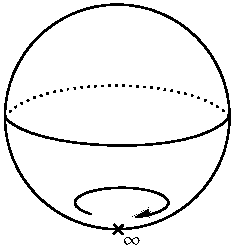
\includegraphics{infty.pdf}
\caption{The monodromy at infinity.}
\label{fig:descendent}
\end{figure}

So the transformation acts on the coordinate $(a,a_D)$ by
\begin{equation}
\left(\begin{array}{cc}
a\\
a_D
\end{array}\right)\mapsto M_\infty
\left(\begin{array}{cc}
a\\
a_D
\end{array}\right)
\end{equation}
where we can easily write down the monodromy matrix $M_\infty$
\begin{equation}
M_{\infty}=\left(\begin{array}{cc}
-1 & 2 \\
0 & -1
\end{array}\right)
\end{equation}

\subsection{Monodromy at Finite $u$}
Now that the infinity point is a singularity, the topological triviality of the whole Coulomb branch implies that there must exist more nontrivial singularities somewhere else. And also, due to the positive-definite metric, the monodromy transformations at finite $u$ form a subgroup of the $SL(2,\vvmathbb{Z})$ and are noncommutative. So except the infinity, there should be two more singularities. 

Since there is a symmetry $u\leftrightarrow -u$, we can assume that the two singularities are at $u= \pm u_0$. The only dynamical scale in this theory is $\Lambda$, we can set $u=\pm\Lambda^2$ up to a constant.

At the singularity of $\mathscr{M}_C$, we will expect new massless degrees of freedom to appear, for example when a massive gauge boson becomes massless. Classically this happens when $u=0$. But quantum mechanically this may shift to a non-zero $u$. While a massive spin-1 multiplet becoming massless can cause inconsistency, the only possible contributions come from spin $\leq 1/2$ multiplets, namely monopoles and dyons (which have both electric and magnetic charge). 

At $u=\Lambda^2$, monopoles become massless, while $a_D\to0$. And at $u=-\Lambda^2$, the dyons become massless with $a+a_D=0$ and $a,a_D\neq 0$.

From the electro-magnetic duality we discovered in sec.\ref{sec:duality}, the original (or electric) theory described by $\Phi$ and $W^\alpha$ is effective at $\infty$. So in the $a_D \to 0$, the dual magnetic coupling is $1/(\mathrm{electric\ coupling})$ and thus the dual magnetic theory is weakly coupled and the description by $\Phi_D$ and $(W_D)_\alpha$ is effective. So we can work in the dual theory where we can adopt perturbative calculations.

\subsection{The Case of $M_+$}
Using one-loop $\beta$-function, we can expand $\tau_D$ around $a_D=0$, which reads
\begin{equation}
\tau_{D} \approx-\frac{\mathrm{i}}{\pi} \ln a_{D}
\end{equation}
at $u=\Lambda^2$, $a_D=0$, $a_D$ is a good coordinate near $u=\Lambda^2$. Then assume $a_D(u)=c(u-\Lambda^2)$ where $c$ is a constant and integrating $\tau_D=\mathrm{d}h_D/\mathrm{d}a_D$ over $a_D$, we can deduce that 
\begin{equation}
a(u)=-h_{D}(u) \approx a_{0}+\frac{\mathrm{i}}{\pi} a_{D} \ln a_{D} \approx a_{0}+\frac{\mathrm{i}}{\pi} c\left(u-\Lambda^2\right) \ln \left(u-\Lambda^2\right)
\end{equation}
This constant $a_0$ cannot be zero or all the electrically charged particles will be massless. When circles around $u=\Lambda^2$,
\begin{equation}
    (u-\Lambda^2)\mapsto \mathrm{e}^{2\pi\mathrm{i}}(u-\Lambda^2)
\end{equation}
$a$ and $a_D$ transforms as
\begin{equation}
\begin{aligned}
a_{D} & \rightarrow a_{D} \\
a & \rightarrow a-2 a_{D}
\end{aligned}
\end{equation}
It is easy to read off the monodromy matrix
\begin{equation}
M_{+}=\left(\begin{array}{cc}
1 & 0 \\
-2 & 1
\end{array}\right)
\end{equation}

\subsection{The Case of $M_-$}
With all of the monodromies taken in the clockwise (or counter clockwise) direction as in figure \ref{fig:finite}, the monodromy obeys $M_\infty=M_+ M_-$. Now it is easy to find that
\begin{equation}
M_{+}=\left(\begin{array}{cc}
-1 & -2 \\
-2 & 3
\end{array}\right)
\end{equation}

\begin{figure}[htbp]
\centering
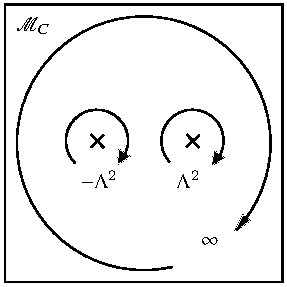
\includegraphics{finite.pdf}
\caption{The monodromy in the strong coupling region.}
\label{fig:finite}
\end{figure}

\subsection{Physical Interpretation}
The singularities on the moduli space of vacua indicates that some massless degrees of freedom exist. Since they cannot be gauge bosons, they are actually monopoles and dyons. At $u=\Lambda^2$ monopoles become massless and at $u=-\Lambda^2$ dyons become massless.


\section{Solution of the Model}
Our final goal here is to determine the prepotential for $\mathcal{N}=2$ $SU(2)$ pure SYM, so we need to perform the integral over $a$ and $a_D$ since $a_D=\mathrm{d}\mathscr{F}(a)/\mathrm{d}a$.

\subsection{Seiberg-Witten Curve}
The three monodromy matrices $M_{\pm}$ and $M_\infty$ do not generate the whole $SL(2,\vvmathbb{Z})$ group. Instead, they generate a congruence group $\Gamma(2)$  consisting of matrices congruent to 1 modulo 2, i.e.
\begin{equation}
    \Gamma(2)=\{M\in SL(2,\vvmathbb{Z}) | M_{ij} = \delta_{ij} (\mathrm{mod} 2) \}
\end{equation}
Moreover, the $u$-plane punctured at $1$, $-1$, and $\infty$ can be regarded as the quotient of the upper half-plane $H$ by $\Gamma(2)$.

The family of curves parametrized by $H/\Gamma(2)$ is given by 
\begin{equation}
    y^3=(x-\Lambda)(x+\Lambda)(x-u).
\end{equation}
This is the famous \textit{Seiberg-Witten curve}, denoted as $E_u$. Here $u$ serves as a complex structure that parametrized these curves i.e. the shape of the curve varies with $u$, see figure \ref{fig:swcurve} for a rough picture.

\begin{figure}[htbp]
\centering
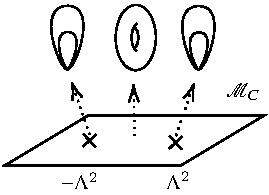
\includegraphics{swcurve.pdf}
\caption{The Seiberg-Witten curves.}
\label{fig:swcurve}
\end{figure}

This curve $E_u$ forms a double cover of the $u$ plane with four branch points $\Lambda$, $-\Lambda$, $u$ and $\infty$. Consider the following way to fix the branch cut: one from $\Lambda$ to $\Lambda$, the other from $u$ to $\infty$. We can easily see that the loop on the $x$-plane that goes around one of the two cuts corresponds to the a-cycle of the torus. On the other hand, a loop that intersects both cuts corresponds to the b-cycle on the torus, see figure \ref{fig:loop}. 

\begin{figure}[htbp]
\centering
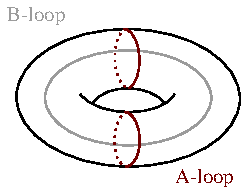
\includegraphics{loop.pdf}
\caption{Schematic illustration of the A-loop and B-loop.}
\label{fig:loop}
\end{figure}

To find out $a$ and $a_D$ on the genus one Riemann surface $E_u$, we pick up two independent one-cycles $A$ and $B$. These one-cycles form a local basis for the first homology group $H^1(E_u,\vvmathbb{C})$. Also, a one-cycle can be paired with elements $\lambda$ from the first cohomology group
\begin{equation}
A,B \rightarrow \oint_{A,B} \lambda
\end{equation}
We can also choose a basis for these one-forms $\lambda$ on $E_u$. Take
\begin{equation}
    \lambda_A=\frac{\mathrm{d}x}{y},\quad\lambda_B=\frac{x\mathrm{d}x}{y}.
\end{equation}
also define
\begin{equation}
    b_{A,B}=\oint_{A,B} \lambda_{A,B}
\end{equation}
Thus 
\begin{equation}
    \tau_u=\frac{b_B}{b_A}
\end{equation}
serves as the modular parameter of the torus which is invariant under $SL(2,\vvmathbb{Z})$ action. Pick an arbitrary section
\begin{equation}
\lambda=a_{A}(u) \lambda_{A}+a_{B}(u) \lambda_{B}
\end{equation}
and claim that
\begin{equation}
a_{D}=\oint_{\gamma_{B}} \lambda, \quad a=\oint_{\gamma_{A}} \lambda
\end{equation}
If $\lambda$ is a form with vanishing residue then, on circling a singularity, $a_D$ and $a$ transform in the right way under $\Gamma(2)$. The above identification of $a_{D}$ and $a$ implies that
\begin{equation}
    \frac{\mathrm{d} a_{D}}{\mathrm{d} u}=\oint_{A} \frac{\mathrm{d} \lambda}{\mathrm{d} u}, \quad \frac{\mathrm{d} a}{\mathrm{d} u}=\oint_{B} \frac{d \lambda}{d u} .
\end{equation}
Since
\begin{equation}
    \tau=\frac{\mathrm{d}a_D}{\mathrm{d}a}=\frac{\mathrm{d}a_D/\mathrm{d}u}{\mathrm{d}a/\mathrm{d}u}
\end{equation}
we make the following identification
\begin{equation}
\tau=\frac{b_{B}}{b_{A}}=\tau_{u} .
\end{equation}
The function $f(u)$ is fixed by the asymptotic behavior of the theory near the singularities on the $u$ plane and is given by $f(u)=-\sqrt{2} / (4 \pi)
$. Then we get the explicit form of $\lambda$ (also called \textit{Seiberg-Witten differential})
\begin{equation}
\label{eq:differential}
\lambda=\frac{\sqrt{2}}{2 \pi} \frac{ \sqrt{x-u}}{\sqrt{x^{2}-1}}\mathrm{d} x
\end{equation}

Now that all the ingredients are ready, recall $\tau=1/\mathscr{F}''$, we can now get the exact form of prepotential $\mathscr{F}$ by integrations!

\subsection{Prepotential from the Curve}
We have the explicit form of \eqref{eq:differential} now but the evaluation involves using a lot of hypergeometric functions. Instead, we use a much simpler method by using \textit{integrable systems}.

It is originally observed in \cite{Gorsky:1995zq} that the Seiberg-Witten solution to $\mathcal{N}=2$ SYM has nontrivial relation with complexified periodic Toda chain. This idea is further developed in \cite{Martinec:1995by,Witten:1997sc}. For a recent review, see \cite{Gorsky:2018ivr}. 

The spectral curve of a $N$-body Toda chain exactly coincides with the Riemann surface introduced in the $SU(N)$ gauge theory. In our $SU(2)$ case, the spectral curve reads 
\begin{equation}
    \Lambda^2(z+\frac{1}{z})=(x^2-u)
\end{equation}
in which $u=p^2-\operatorname{cosh}q$ with $p,q$ generalized momentum and coordinate of the periodic Toda system. The action variable
\begin{equation}
a=\oint p \mathrm{~d} q=\oint \sqrt{u-\cosh q} \mathrm{~d} q=\oint x \frac{\mathrm{d} z}{z}, \quad \lambda=x \frac{\mathrm{d} z}{z}
\end{equation}
with $z=\mathrm{e}^q$. Around different loops this action variable will coincide with $a$ and $a_D$.
\begin{equation}
    a=\frac{1}{2\pi\mathrm{i}}\oint_A\lambda,\quad a_D=\frac{1}{2\pi\mathrm{i}}\oint_B\lambda.
\end{equation}

Since $a_D=\partial\mathscr{F}(a)/da$, integrating twice and we get the expansion of $\mathscr{F}$ as
\begin{equation}
\label{eq:prep2}
2 \pi i \mathscr{F}(a)=-4 a^{2} \log \frac{a}{\Lambda}+\sum_{k=1}^{\infty} c_{k} \frac{\Lambda^{4 k}}{a^{4 k-2}}
\end{equation}
Now we follow \cite{Chan:1999gj,Tac15} to determine the numerical factor $c_k$.

We adopt the renormalization group relation in \cite{Matone:1995rx}, which is 
\begin{equation}
\label{eq:RG}
2 \pi i \Lambda \frac{\partial}{\partial \Lambda} \mathscr{F}(a, \Lambda)=4 u
\end{equation}
Set $u=\tilde{a}^2$ with $\tilde{a}$ the renormalized VEV, we can perform the integration as follows
\begin{equation}
\begin{aligned}
a(\tilde{a}) &=\frac{1}{2 \pi i} \oint_{A} \lambda=\frac{1}{2 \pi i} \oint_{A}\left(\sum_{l=0}^{\infty}\left(z+\frac{1}{z}\right)^{l} \frac{(-1)^{l}(2 l) !}{(1-2 l)(l !)^{2} 2^{2 l}} \frac{\Lambda^{2 l}}{a^{2 l-1}}\right) \frac{\mathrm{d} z}{z} \\
&=\tilde{a} \sum_{k=0}^{\infty} \frac{\Lambda^{4 k}}{\tilde{a}^{4 k}} \frac{1}{(1-4 k) 2^{4 k}} \frac{(4 k) !}{(2 k) ! k ! k !}.
\end{aligned}
\end{equation}

A self-consistent calculation is to substitute \eqref{eq:prep2} into \eqref{eq:RG}, then we have 
\begin{equation}
a^{2}\left(1+\sum_{k=1}^{\infty} k c_{k} \frac{\Lambda^{4 k}}{a^{4 k}}\right)=\tilde{a}^{2}
\end{equation}
Then by comparing coefficients, we can easily see the first few terms of the instanton corrections
\begin{equation}
\label{eq:coeff}
c_{1}=\frac{1}{2}, c_{2}=\frac{5}{64}, c_{3}=\frac{3}{64}, c_{4}=\frac{1469}{32768}, \ldots
\end{equation}

\section{Instanton counting}
In the seminal paper \cite{Nekrasov:2002qd}, Nekrasov purposed a new way to derive the prepotential of $\mathcal{N}=2$ $SU(2)$ pure SYM directly from the so-called \emph{instanton counting}. By considering a closely related 5d gauge theory and making use of equivariant localization, the prepotential can be precisely recovered. We will review the $SU(2)$ SYM case following \cite{Tac15} and then extend it to the $SU(N)$ SYM.

\subsection{From 5d to 4d}
To perform instanton counting for a 4d gauge theory with gauge group $G$, we first consider a 5d gauge theory of the same gauge group. Then, when we compactify this theory on $S^1$ with radius $\beta$ and then take the zero-radius limit $\beta\to 0$, we can recover the 4d theory.

Now we introduce the $\Omega$-background. Since the 5d theory live on $\vvmathbb{R}^5$, regard $\vvmathbb{R}^5$ as $\vvmathbb{C}^2\times\vvmathbb{R}$ with complex coordinate $(z_1,z_2)$ and real coordinate $x_5$. Then we make the following identification
\begin{equation}
\left(z_{1}, z_{2}, x_{5}\right) \sim\left(z_{1} e^{\mathrm{i} \beta \epsilon_{1}}, z_{2} e^{\mathrm{i} \beta \epsilon_{2}}, x_{5}+\beta\right)
\end{equation}

To preserve supersymmetry, we need to introduce a corresponding $SU(2)_R$ rotation
\begin{equation}
\operatorname{diag}\left(e^{\mathrm{i} \beta\left(\epsilon_{1}+\epsilon_{2}\right) / 2}, e^{-\mathrm{i} \beta\left(\epsilon_{1}+\epsilon_{2}\right) / 2}\right) \in SU(2)_{R}
\end{equation}
and a gauge rotation $\mathrm{e}^{\mathrm{i}\beta \vec{a}}\in G$, where $\vec{a}$ an element of Lie algebra of $G$.

Regarding the $x_5$ direction as the time direction, then the system on $\vvmathbb{R}^4$ is forced to rotate by $\beta\epsilon_{1,2}$. So any excitations far from the origin are suppressed. The effective scale of the system is $1/\epsilon_1\epsilon_2$ and thus the partition function of the system can be written as 
\begin{equation}
\log Z\left(\epsilon_{1,2}, \tau_{U V} ; \vec{a}\right)=\frac{1}{\epsilon_{1} \epsilon_{2}} F\left(\tau_{U V} ; \vec{a}\right)+\text { terms less singular in } \epsilon_{1,2} .
\end{equation}
in which $F$ stands for the density of free energy, $\tau_{UV}$ is the 5d coupling constant constructed from the 't Hooft coupling $g_{UV5}$. The gauge theory part of the 5d Lagrangian can be written as
\begin{equation}
\int d x_{5} \int d^{4} x \frac{1}{2 g_{U V 5}^{2}} \operatorname{tr} F_{\mu \nu} F^{\mu \nu}.
\end{equation}
By integrating out $x_5$ we can get the coupling
\begin{equation}
    \tau_{UV}=\beta\frac{4\pi\mathrm{i}}{g_{U V 5}^{2}}
\end{equation}

We here claim that this free energy $\mathcal{F}$ equals the prepotential:
\begin{equation}
\label{eq:prepcount}
    2 \pi \mathrm{i} \mathscr{F}\left(\tau_{U V} ; \vec{a}\right)=F\left(\tau_{U V} ; \vec{a}\right)=\lim _{\epsilon_{1,2} \rightarrow 0} \epsilon_{1} \epsilon_{2} \log Z\left(\tau_{U V} ; \vec{a}\right)
\end{equation}
So after taking the limit $\beta \rightarrow 0$, we can then get the prepotential. For proof of this claim, see \cite{Nekrasov:2002qd}.

\subsection{Reduction to Supersymmetric Quantum Mechanics}
The perturbative part of the partition corresponds to the one-loop part in the prepotential \eqref{eq:pre}. What we are interested in is the nonperturbative contributions from instantons. The energy of a gauge field can be written as
\begin{equation}
\int d^{4} x \frac{1}{2 g_{U V 5}^{2}} \operatorname{tr} F_{\mu \nu} F^{\mu \nu}
\end{equation}
which is bound from below by $8\pi^2\abs{k}=g_{UV5}^2$, and $k$ the instanton number.

The instanton configurations can be described by the $k$ instanton moduli space $M_k$. Given a point $p\in M_k$, we have an instanton solution $F_{\mu\nu}(x_{1,2,3,4};p)$ for $\mu,\nu=1,2,3,4$. As the time $t=x_5$ changes, the shape of the instanton varies, forming a path $p(t)$ in $M_k$. 

Then we can rewrite the 5d action for gauge theory as follows
\begin{equation}
\int d t \int d^{4} x \frac{1}{2 g_{U V 5}^{2}} \operatorname{tr} F_{\mu \nu} F^{\mu \nu}=\int d t\left(\frac{8 \pi^{2}}{2 g_{U V 5}^{2}}+G_{I J}(p) \partial_{t} p^{I}(t) \partial_{t} p^{J}(t)\right).
\end{equation}
The first term on the right-hand side comes from the part with $x_5$, while the second term only consists of $x_{1,2,3,4}$. The index $I,J$ runs from $1$ to $\dim M_k$, and $G_{IJ}$ serves as the metric on $M_k$.

Since anti-instantons only contribute to the anti-holomorphic part of the partition function, we can safely write 
\begin{equation}
\label{eq:shift}
    Z_{\mathrm{non-pert.}}=\sum_{k=0}^{\infty}Z_k,\quad Z_{k}=e^{2 \pi i \tau_{U V} k} \tilde{Z}_{k}.
\end{equation}
where the constant energy shift comes from the terms with $x_5$ dependence, and $\tilde{Z}_{k}$ is the partition function of the supersymmetric quantum mechanics on $M_k$ with the zero energy at the ground state.

\subsection{Instanton Counting of Seiberg-Witten Theory}
Now we start to compute the instanton partition function (or Nekrasov partition function) for $SU(2)$ pure SYM.

\subsection{$k=0$ Case}
In $k=0$ case the moduli space $M_0$ is a single point. It is a 1d Hilbert space with zero Hamiltonian, so we have 
\begin{equation}
    Z_0=1.
\end{equation}

\subsection{$k=1$ Case}
The $k=1$ moduli space is a little bit more complicated. We need to first specify its center-of-mass position in $\vvmathbb{C}^2$ (or $\vvmathbb{R}^4$). Also, An $SU(2)$ instanton has a size (radius) $\rho$, which is a non-negative real number, and a gauge direction in the group manifold. Since the gauge direction takes values in the $SO(3)$ group manifold, which is $\vvmathbb{R}P^2=S^3/\vvmathbb{Z}_2$. Combining with $\rho$ we get $\vvmathbb{C}^2/\vvmathbb{Z}_2$.

Then, the coordinate on the moduli space is $(z_1,z_2,u,v)$ with $(u,v)\sim-(u,v)$. Under the rotation by $\beta\epsilon_{1,2}$, the coordinate transforms by
\begin{equation}
\left(z_{1}, z_{2}, u, v\right) \mapsto\left(e^{\mathrm{i} \beta \epsilon_{1}} z_{1}, e^{\mathrm{i} \beta \epsilon_{2}} z_{2}, e^{\mathrm{i} \beta\left(\epsilon_{1}+\epsilon_{2}\right) / 2} u, e^{\mathrm{i} \beta\left(\epsilon_{1}+\epsilon_{2}\right) / 2} v\right).
\end{equation}
Under gauge rotation 
\begin{equation}
\operatorname{diag}\left(e^{\mathrm{i} \beta a}, e^{-\mathrm{i} \beta a}\right) \in SU(2)
\end{equation}
$z_1,z_2$ remain unchanged, but $u,v$ will transform as follows
\begin{equation}
(u, v) \mapsto\left(e^{\mathrm{i} \beta a} u, e^{-\mathrm{i} \beta a} v\right).
\end{equation}

Since the supersymmetric wavefunctions are holomorphic functions of $z_1$, The state whose wavefunction is $z_1^n$ gets multiplied by $e^{-\mathrm{i} \beta \epsilon_1}$ by the spatial rotation. The partition function of the degrees of freedom on the motion described by $z_1$ is by tracing over the corresponding Hilbert space. Therefore, this part contributes
\begin{equation}
\sum_{n=0}^{\infty} e^{\mathrm{i} n \beta \epsilon_{1}}=\frac{1}{1-e^{\mathrm{i} \beta \epsilon_{1}}}
\end{equation}
By similar analysis we can also write down the contributions of $z_2$ and $(u,v)$, but notice that there is a constraint $(u,v)\sim-(u,v)$ so that for wave functions of the form $u^n v^m$, only even $n+m$ survives. Therefore the complete contributions are 
\begin{equation}
\begin{aligned}
\sum_{n \geq 0, m \geq 0, n+m: \text { even }} e^{\mathrm{i} n \beta\left(\left(\epsilon_{1}+\epsilon_{2}\right) / 2+a\right)} e^{\mathrm{i} m \beta\left(\left(\epsilon_{1}+\epsilon_{2}\right) / 2-a\right)} \\
= \frac{1+e^{\mathrm{i} \beta\left(\epsilon_{1}+\epsilon_{2}\right)}}{\left(1-e^{\mathrm{i} \beta\left(\epsilon_{1}+\epsilon_{2}+2 a\right)}\right)\left(1-e^{\mathrm{i} \beta\left(\epsilon_{1}+\epsilon_{2}-2 a\right)}\right)} .
\end{aligned}
\end{equation}
Finally, combining the constant energy shift in\eqref{eq:shift}, the one-instanton contribution is
\begin{equation}
Z_{1}=e^{2 \pi \mathrm{i} \tau_{U V}} \frac{1}{1-e^{\mathrm{i} \beta \epsilon_{1}}} \frac{1}{1-e^{\mathrm{i} \beta \epsilon_{2}}} \frac{1+e^{\mathrm{i} \beta\left(\epsilon_{1}+\epsilon_{2}\right)}}{\left(1-e^{\mathrm{i} \beta\left(\epsilon_{1}+\epsilon_{2}+2 a\right)}\right)\left(1-e^{\mathrm{i} \beta\left(\epsilon_{1}+\epsilon_{2}-2 a\right)}\right)} .
\end{equation}

Next step would be taking the $\beta\to 0$ limit. By one-loop running for $\tau_{UV}$, we can expect that $e^{2 \pi \mathrm{i}}\sim \beta^4$ by identifying $\Lambda \sim \beta^{-1}$ which makes this limit reasonable. 

Let us take the $\beta\to 0$ limit fixing
\begin{equation}
\Lambda^{4}:=\beta^{-4} e^{2 \pi i \tau_{U V}}
\end{equation}
The limit is then
\begin{equation}
Z_{1} \rightarrow \Lambda^{4} \frac{1}{2} \frac{1}{\epsilon_{1}} \frac{1}{\epsilon_{2}} \frac{1}{\left(\epsilon_{1}+\epsilon_{2}\right) / 2+a} \frac{1}{\left(\epsilon_{1}+\epsilon_{2}\right) / 2-a}
\end{equation}
Plugging into \eqref{eq:prepcount}, we have 
\begin{equation}
\label{eq:k1}
2 \pi \mathrm{i} \mathscr{F}_{\text {non-pert. }}=\lim _{\epsilon_{1,2} \rightarrow 0} \epsilon_{1} \epsilon_{2} \log \left(1+e^{2 \pi \mathrm{i} \tau_{U V}} Z_{1}+\cdots\right)=\frac{1}{2} \frac{\Lambda^{4}}{a^{2}}+\cdots .
\end{equation}
which coincide with the corresponding term in \eqref{eq:coeff}. 

Similar computation can be done for any $k$, and the result can be summarized in a combinatorial formula
\begin{equation}
\begin{aligned}
\label{eq:young}
Z_{k}= &\sum_{Y_{1}, Y_{2}} \prod_{n, m=1}^{2} \prod_{s \in Y_{n}} \frac{1}{1-e^{\mathrm{i} \beta\left(-L_{Y_{m}}(s) \epsilon_{1}+\left(A_{Y_{n}}(s)+1\right) \epsilon_{2}+a_{m}-a_{n}\right)}}\\
&\prod_{t \in Y_{m}} \frac{1}{1-e^{\mathrm{i} \beta\left(\left(L_{Y_{n}}(t)+1\right) \epsilon_{1}-A_{Y_{m}}(s) \epsilon_{2}+a_{m}-a_{n}\right)}} .
\end{aligned}
\end{equation}
where the sum runs over pairs $(Y_1,Y_2)$ of Young diagrams with the number of total boxes being $k$, $s \in Y$ denotes that $s$ is a box in a Young diagram $Y$, and finally the functions $A_Y(s)$ and $L_Y(s)$ are the arm length and the leg length of the box $s$ in a Young diagram $Y$.

\begin{figure}[htbp]
\centering
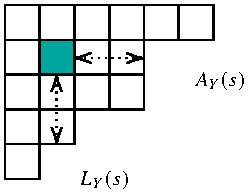
\includegraphics{young.pdf}
\caption{The definition of the arm length and the leg length in a Young diagram.}
\label{fig:young}
\end{figure}

For a mathematical proof that \eqref{eq:young} recovers the Seiberg-Witten curve, see Okounkov-Nekrasov \cite{Okounkov:2006wj} for a combinatorial proof, Nakajima-Yohsioka \cite{Nakajima:2003pg} by blow-up method on instanton moduli space and Braverman-Etingof \cite{Braverman:2004cr} using affine Lie algebra.

By summing over the contributing pairs of diagrams $(\,\tikzset{every picture/.style={line width=0.75pt}}\begin{tikzpicture}[x=0.75pt,y=0.75pt,yscale=-1,xscale=1]\draw   (20.67,21.67) -- (29.83,21.67) -- (29.83,30.83) -- (20.67,30.83) -- cycle ;\end{tikzpicture}\,,0)$ and $(0,\tikzset{every picture/.style={line width=0.75pt}}\begin{tikzpicture}[x=0.75pt,y=0.75pt,yscale=-1,xscale=1]\draw   (20.67,21.67) -- (29.83,21.67) -- (29.83,30.83) -- (20.67,30.83) -- cycle ;\end{tikzpicture}\,)$ we can easily recover the result in \eqref{eq:k1}.

For $k=2$ case the contributing diagrams are 
$(\tikzset{every picture/.style={line width=0.75pt}} %set default line width to 0.75pt        
\begin{tikzpicture}[x=0.75pt,y=0.75pt,yscale=-1,xscale=1, baseline=(XXXX.south) ]
\path (0,22);\path (12.990839004516602,0);\draw    ($(current bounding box.center)+(0,0.3em)$) node [anchor=south] (XXXX) {};
%Shape: Square [id:dp21359378593647516] 
\draw   (2,10.85) -- (11.15,10.85) -- (11.15,20) -- (2,20) -- cycle ;
%Shape: Square [id:dp1169763623479887] 
\draw   (2,1.69) -- (11.15,1.69) -- (11.15,10.85) -- (2,10.85) -- cycle ;
\end{tikzpicture}
,0 )$, $(\tikzset{every picture/.style={line width=0.75pt}} %set default line width to 0.75pt        
\begin{tikzpicture}[x=0.75pt,y=0.75pt,yscale=-1,xscale=1, baseline=(XXXX.south) ]
\path (0,13);\path (22.66666666666667,0);\draw    ($(current bounding box.center)+(0,0.3em)$) node [anchor=south] (XXXX) {};
%Shape: Square [id:dp5959708258303704] 
\draw   (11.15,1.69) -- (20.31,1.69) -- (20.31,10.85) -- (11.15,10.85) -- cycle ;
%Shape: Square [id:dp4837801742553729] 
\draw   (2,1.69) -- (11.15,1.69) -- (11.15,10.85) -- (2,10.85) -- cycle ;
\end{tikzpicture}
,0 )$, $(\,\tikzset{every picture/.style={line width=0.75pt}}\begin{tikzpicture}[x=0.75pt,y=0.75pt,yscale=-1,xscale=1]\draw   (20.67,21.67) -- (29.83,21.67) -- (29.83,30.83) -- (20.67,30.83) -- cycle ;\end{tikzpicture}\,,\tikzset{every picture/.style={line width=0.75pt}}\begin{tikzpicture}[x=0.75pt,y=0.75pt,yscale=-1,xscale=1]\draw   (20.67,21.67) -- (29.83,21.67) -- (29.83,30.83) -- (20.67,30.83) -- cycle ;\end{tikzpicture}\,)$, $(0,\tikzset{every picture/.style={line width=0.75pt}} %set default line width to 0.75pt        
\begin{tikzpicture}[x=0.75pt,y=0.75pt,yscale=-1,xscale=1, baseline=(XXXX.south) ]
\path (0,13);\path (22.66666666666667,0);\draw    ($(current bounding box.center)+(0,0.3em)$) node [anchor=south] (XXXX) {};
%Shape: Square [id:dp21771453172207633] 
\draw   (11.15,1.69) -- (20.31,1.69) -- (20.31,10.85) -- (11.15,10.85) -- cycle ;
%Shape: Square [id:dp155318443439439] 
\draw   (2,1.69) -- (11.15,1.69) -- (11.15,10.85) -- (2,10.85) -- cycle ;
\end{tikzpicture}
)$, $(0,\tikzset{every picture/.style={line width=0.75pt}} %set default line width to 0.75pt        
\begin{tikzpicture}[x=0.75pt,y=0.75pt,yscale=-1,xscale=1, baseline=(XXXX.south) ]
\path (0,22);\path (12.990839004516602,0);\draw    ($(current bounding box.center)+(0,0.3em)$) node [anchor=south] (XXXX) {};
%Shape: Square [id:dp22287086838156656] 
\draw   (2,10.85) -- (11.15,10.85) -- (11.15,20) -- (2,20) -- cycle ;
%Shape: Square [id:dp6625795647603105] 
\draw   (2,1.69) -- (11.15,1.69) -- (11.15,10.85) -- (2,10.85) -- cycle ;
\end{tikzpicture}
)$, the computation gives that
\begin{equation}
Z_{2} \rightarrow \Lambda^{8} \frac{\left(8\left(\epsilon_{1}+\epsilon_{2}\right)^{2}+\epsilon_{1} \epsilon_{2}-8 a^{2}\right)}{\epsilon_{1}^{2} \epsilon_{2}^{2}\left(\left(\epsilon_{1}+\epsilon_{2}\right)^{2}-4 a^{2}\right)\left(\left(2 \epsilon_{1}+\epsilon_{2}\right)^{2}-4 a^{2}\right)\left(\left(\epsilon_{1}+2 \epsilon_{2}\right)^{2}-4 a^{2}\right)}
\end{equation}
in the limit $\beta \to 0$.

Plugging into \eqref{eq:prepcount} we can conclude that
\begin{equation}
\begin{aligned}
2 \pi i \mathscr{F}_{\text {non-pert }} &=\lim _{\epsilon_{1,2} \rightarrow 0} \epsilon_{1} \epsilon_{2} \log \left(1+Z_{1}+Z_{2}+\cdots\right) \\
&=\lim _{\epsilon_{1,2} \rightarrow 0} \epsilon_{1} \epsilon_{2}\left(Z_{1}+\left(Z_{2}-\frac{1}{2} Z_{1}^{2}\right)+\cdots\right) \\
&=\frac{1}{2} \frac{\Lambda^{4}}{a^{2}}+\frac{5}{64} \frac{\Lambda^{8}}{a^{6}}+\cdots
\end{aligned}
\end{equation}
which matches with the first two terms in \eqref{eq:coeff}.

\section{Extending to Higher Rank}
Now we extend the discussion to higher rank i.e. the $SU(N)$ case. The Seiberg-Witten-like analysis is considered in \cite{Argyres:1994xh} and \cite{Klemm:1994qs}. Some parts of this chapter are modified from Tachikawa's master thesis.

\subsection{The Curve}
For this case, the gauge group is completely broken into $U(1)^{N-1}$, and the metric $\operatorname{Im}\tau_{ij}$ should be positive definite. The electro-magnetic duality group extends to $Sp(2N-2,\vvmathbb{Z})$ accordingly.

A natural extension of the original Seiberg-Witten curve is
\begin{equation}
    y^2=P(x)^2-\Lambda^{2N}
\end{equation}
with
\begin{equation}
    P(x)=\langle\operatorname{det}(x-\phi)\rangle=\sum_p u_{p} x^{n-p}.
\end{equation}
so $a_k$ and $a_{D,k}$ takes the form
\begin{equation}
    a_k=\frac{1}{2\pi\mathrm{i}}\oint_{A_k}\lambda,\quad a_{D,k}=\frac{1}{2\pi\mathrm{i}}\oint_{B_k}\lambda.
\end{equation}
And the Seiberg-Witten differential is now
\begin{equation}
   \lambda=\frac{x\mathrm{d}P(x)}{y}.
\end{equation}

Next, we shall determine the prepotential by actually doing this integral. One way is to solve the Picard-Fuchs equations that $a$ and $a_D$ satisfy. But a simpler method is to determine the coefficients recursively, following \cite{Chan:1999gj,DHoker:1996pva}.

\subsection{Classical Moduli}
Now we first show without proof the form of $a_i$ in terms of the classical moduli $\tilde{a}_i$ appearing in the definition of the curves
\begin{equation}
    P(x)=\prod_i (x-\tilde{a}_i)
\end{equation}
The quantum correction is of the form
\begin{equation}
\label{eq:classical}
   a_{k}=\tilde{a}_{k}+\sum_{m=1}^{\infty} \frac{\Lambda^{2 m}}{2^{2 m}(m !)^{2}}\left(\frac{\partial}{\partial \tilde{a}_{k}}\right)^{2 m-1} S_{k}\left(\tilde{a}_{k}\right)^{m}, 
\end{equation}
where
\begin{equation}
   S_{k}(x)=\frac{\Lambda^{2(N-1)}}{\prod_{i \neq k}\left(x-\tilde{a}_{i}\right)^{2}} . 
\end{equation}

\subsection{Linear Recursion Relation}
By using the renormalization group equation derived in \cite{Matone:1995rx} for $SU(2)$ and in \cite{Eguchi:1995jh,Sonnenschein:1995hv} for $SU(N)$
\begin{equation}
\label{eq:RGEN}
\Lambda \frac{\partial \mathscr{F}}{\partial \Lambda}=\frac{N}{\pi i} \sum_k \tilde{a}_{k}^{2}
\end{equation}

First, we calculate $\Lambda(\partial\mathscr{F}/\partial\Lambda)$ by substitute the full form of prepotential 
\begin{equation}
\mathscr{F}=\frac{N}{\pi \mathrm{i}} \sum_k a_{k}^{2}+\frac{\mathrm{i}}{4 \pi} \sum_{i<j}\left(a_{i}-a_{j}\right)^{2} \log \frac{\left(a_{i}-a_{j}\right)^{2}}{\Lambda^{2}}+\sum_{m=1}^{\infty} \frac{\Lambda^{2 N m}}{2 m \pi \mathrm{i}} c_m(a)
\end{equation}
into \eqref{eq:RGEN}, we get 
\begin{equation}
\sum_k \tilde{a}_{k}^{2}=\sum_k a_{k}^{2}+\sum_{m=1}^{\infty} \Lambda^{2 N m} c_m(a)
\end{equation}
Then, substituting $a_k$ by $\tilde{a}_k$
\begin{equation}
0=\sum_{k}\left(\sum_{m=0}^{\infty} \Lambda^{2 N m} \Delta_{k}^{(m)}(\tilde{a})\right)^{2}-\sum_{k}\left(\Delta_{k}^{(0)}(\tilde{a})\right)^{2}+\sum_{m=1}^{\infty} \Lambda^{2 N m} c_{m}\left(\sum_{n=0}^{\infty} \Lambda^{2 N n} \Delta_{k}^{(n)}(\tilde{a})\right)
\end{equation}
where we define
\begin{equation}
\Delta_{k}^{(m)}(x)=\frac{1}{2^{2 m}(m !)^{2}}\left(\frac{\partial}{\partial x}\right)^{2 m-1} S_{k}(x)^{m},\quad \Delta_{k}^{(0)}(x)=\tilde{a}_k.
\end{equation}
With this, we can compute to any order the instanton correction $c_m$ recursively, by substituting $\tilde{a}_k$s with $a_k$s.

The first several contributions are 
\begin{equation}
\begin{aligned}
\label{eq:recursion}
-c_1=& \sum_k 2 \Delta_{k}^{(0)} \Delta_{k}^{(1)} \\
-c_2=& \sum_k \left(2 \Delta_{k}^{(0)} \Delta_{k}^{(2)}+\left(\Delta_{k}^{(1)}\right)^{2}\right)+\sum_k  \Delta_{k}^{(1)} \frac{\partial}{\partial a_{k}} c_{1} \\
-c_3=& \sum_k \left(2 \Delta_{k}^{(0)} \Delta_{k}^{(3)}+2 \Delta_{k}^{(1)} \Delta_{k}^{(2)}\right) \\
&+\sum_k \left(\Delta_{k}^{(1)} \frac{\partial}{\partial a_{k}} c_2+\Delta_{k}^{(2)} \frac{\partial}{\partial a_{k}} c_1\right)+\frac{1}{2} \sum_{k,l} \Delta_{k}^{(1)} \Delta_{l}^{(1)} \frac{\partial^{2}}{\partial a_{k} \partial a_{l}} c_1
\end{aligned}
\end{equation}

\subsection{Nekrasov's Formula}
The instanton counting for $SU(N)$ is similar to the $SU(2)$ case. Note that we now have $N$ Young tables and for a $k$-instanton contribution we require the total number of boxes in all Young tables is $k$. Here we present the formula without derivation, for a detailed calculation, see \cite{Nekrasov:2002qd,Moore:1997dj}. By setting $\epsilon_1=-\epsilon_2=\epsilon$, the 5d partition function reads

\begin{equation}
\begin{aligned}
Z &=\sum_{k} q^{k} \sum_{\left(Y_{1, \ldots}, \ldots, Y_{N}\right), \Sigma \# Y_{i}=k} \sum_{i, j} \sum_{s \in Y_{i} \cup Y_{j}} \\
& \frac{1}{\sinh \frac{\beta}{2}\left(a_{i}-a_{j}+\epsilon\left(-L_{Y_{j}}(s)-A_{Y_{i}}(s)-1\right)\right)} \frac{1}{\sinh \frac{\beta}{2}\left(a_{i}-a_{j}+\epsilon\left(L_{Y_{i}}(s)+A_{Y_{j}}(s)+1\right)\right)} \\
&=\sum_{k} q^{k} \sum_{\left(Y_{1}, \ldots, Y_{N}\right), \Sigma \# Y_{i}=k} \sum_{(i, m) \neq(j, n)} \frac{\sinh \frac{\beta}{2}\left(a_{i}-a_{j}+\epsilon\left(y_{i, n}-y_{j, m}+m-n\right)\right)}{\sinh \frac{\beta}{2}\left(a_{i}-a_{j}+\epsilon(m-n)\right)}
\end{aligned}
\end{equation}
in which $y_{i,m}$ is the total number of boxes in the $m$-th row of the $i$-th Young table $Y_i$. 

Taking $\beta\to 0$ limit with Coulomb branch parameters $a_i$ fixed, we get the 4d partition function
\begin{equation}
Z=\sum_{k} \Lambda^{2 N k} \sum_{\left(Y_{1}, \ldots, Y_{N}\right), \Sigma \# Y_{i}=k} \sum_{(i, m) \neq(j, n)}
\frac{\left(a_{i}-a_{j}+\epsilon\left(y_{i, n}-y_{j, m}+m-n\right)\right)}{\left(a_{i}-a_{j}+\epsilon(m-n)\right)}.
\end{equation}

Recall the prepotential is related to the instanton partition function via
\begin{equation}
\mathscr{F}=\lim _{\epsilon \rightarrow 0} \epsilon^{2} \log Z
\end{equation}
Up to two instantons, the results are 
\begin{equation}
\begin{aligned}
c_1=& \frac{1}{2} \sum_{l} \prod_{k \neq l} \frac{1}{\left(a_{k}-a_{l}\right)^{2}}, \\
c_2=& \frac{1}{4} \sum_{l} \sum_{k \neq l, m \neq l} \frac{1}{a_{k}-a_{l}} \frac{1}{a_{m}-a_{l}} \prod_{k \neq l} \frac{1}{\left(a_{k}-a_{l}\right)^{2}}+\frac{3}{8} \sum_{l} \sum_{k \neq l} \frac{1}{\left(a_{k}-a_{l}\right)^{2}} \prod_{k \neq l} \frac{1}{\left(a_{k}-a_{l}\right)^{2}} \\
&+\frac{1}{4} \sum_{l \neq m} \frac{1}{\left(a_{l}-a_{m}\right)^{2}} \prod_{k \neq l} \frac{1}{\left(a_{k}-a_{l}\right)^{2}} \prod_{k \neq m} \frac{1}{\left(a_{k}-a_{m}\right)^{2}} .
\end{aligned}
\end{equation}
This exactly agrees with the result in \eqref{eq:recursion}. For larger $k$, writing down the explicit expression is relatively hard. But we can verify this relation to arbitrarily high order using numerical methods. In the file attached, we numerically verified the result of the Seiberg-Witten curve with instanton partition function to $k=4$ case.

\bibliographystyle{amsalpha}
\bibliography{main.bib}


\end{document}
